\documentclass[xcolor=dvipsnames]{beamer}

\usetheme{Frankfurt}
\usepackage{paralist}
\usecolortheme[RGB={0,104,139}]{structure}%deepskyblue
%\usecolortheme[named=Maroon]{structure}

\title[Cloud based IT Infra with Central Identity]{Cloud based IT Infra with Central Identity}
\subtitle{\{Project reboot\} - Phase I  }

\author{ \underline{Project Guide} \\ \hspace{2mm} \\ \small{ T. Chandra Shekar }  }
\institute{ \underline{Presenting by} \\ \hspace{2mm} \\ \textit {Team r3b00+ }  \\ \hspace{4mm} \\ \textit{Dept. of CSE, RGUKT - Nuzvid}}

\begin{document}


\begin{frame}
\titlepage
\end{frame}

\section{About us}
\begin{frame}{About us}

\small
\begin{center}
We are from team \textit{r3b00+}  \{reboot\} \\ \hspace{4cm} \\
\begin{tabular}{l  l }
T. Aneesh Kumar & N090247   \\
P. Nageswarao  & N091030  \\
P. Anesh  & N090977 \\
P. Jyothi Ram & N090990 \\
K. Naresh Chowdary  & N090331 \\
N. Venkata Sateesh  & N090935 \\
M. Sanyasi Rao & N090891  
\end{tabular}


\end{center}


\end{frame}
 
\setcounter{page}{1}
\section{Objective}
\begin{frame}{Objective}
To construct new Cloud based IT Infra with Central Identity.
\end{frame}

\begin{frame}{Objective Continued ...}

The main objective of ``Cloud based IT Infra with Central Identity'' is to utilize exisiting hardware, turn them into private clouds and access all of its services using 
Central Identity, which can be available to third party developers as API with dynamic role management and service endpoints. \newline

New private cloud based IT Infra is aimed to develop using some opensource tools like OpenStack, NFS, LDAP, Ubuntu and etc \newline

Expecting to serve with high computational virtual machines to the research, academic, learning purpose, virtal labs rather than dedicated lab hardware.
\end{frame}

\section{Motivation}
\begin{frame}{Motivation}

\begin{itemize}
	\item No Central Identity, Central Storage \& High capacity hardware resource pool.
	\item Failed to maintain large user load web services like ONB, Exam servers, etc.
	\item Dedicated computer course labs like Matlab, VLSI, etc.
	\item No proper Web Application Security \& Standards.
	\item Inadequate resource requirements for Research.
\end{itemize}

\end{frame}



\section{Proposed System}
\begin{frame}{Users \& IT Services}
We are grouping all IT Services that are required for University into one and identifing the user who will going to use them. All Users are catagorized into 4 groups $ ^{[1]}$
	
	\begin{itemize}
	\item Studens, Developers, Staff, faculty \& Researches
	\end{itemize}
\begin{figure}[H]
\begin{center}
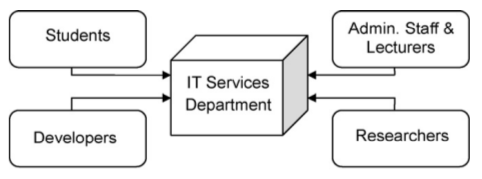
\includegraphics[width=5cm]{./it.png}
\caption{ Simplified structure of the main users of IT services. \label{fig:Simplified structure of the main users of IT services. }}
\end{center}
\end{figure}
	
\end{frame}

\begin{frame}{Cloud Infrastructures}
All University IT Services are deployed in a private cloud, constructed over exsiting infrastructure, that can be browdly viewed as 
	
\begin{figure}[H]
\begin{center}
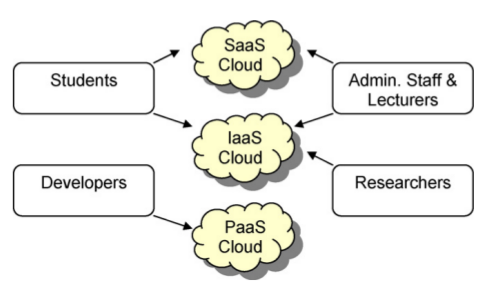
\includegraphics[width=7cm]{./it2.png}
\caption{ IT Services and Users in Cloud Computing\label{fig:IT Services and Users in Cloud Computing }}
\end{center}
\end{figure}	
	
	
\end{frame}

\begin{frame}{Proposed System -  Main Components}
\begin{itemize}
	\item Central Identiy 
	\begin{itemize}
		\item Single Sign on
		\item Fedarated Identity
		\item Dynamic Role Based Access Control
		\item REST API to third party
	\end{itemize}
	\item Network Components Configurations
	\begin{itemize}
		\item AAA, LDAP, NFS
	\end{itemize}
	\item Cloud Infrastructure
	\begin{itemize}
		\item Cloud Computing, Private Cloud, Open source tools
	\end{itemize}
\end{itemize}
\end{frame}

\section{Cloud Computing}
\begin{frame}{Cloud Computing - Definition }

What is Cloud Computing ...? \\
\hspace{4cm} \\
\textit{``Cloud computing is a model for enabling convenient, on-
demand network access to a shared pool of configurable
computing resources (e.g., networks, servers, storage,
applications, and services) that can be rapidly provisioned
and released with minimal management effort or service
provider interaction''} $ ^{[1]} $

\end{frame}

\begin{frame} {Cloud Computing - Characteristics }
One can define Cloud Computing with essential characteristics like

\begin{itemize}
\item On-demand self-service
\item Broad network access
\item Resource pooling
\item Rapid elasticity
\item Measured Service
\end{itemize}
\end{frame}

\begin{frame}{Cloud Computing - Servcice Models }

If we providing any thing as a service comes, that will comes into Cloud Computing. Various Service Delivery Models listed bellow.

\begin{itemize}
\item Software as a Service (SaaS) 
%\begin{itemize}
%	\item Google Docs, Photo editors, Calculators, etc
%\end{itemize}
\item Platform as a Service (PaaS)
%\begin{itemize}
%	\item Harkoo, Aneka, Google App engine, etc
%\end{itemize}
\item Infrastructure as a Service (IaaS)
%\begin{itemize}
%	\item AWS, Openstack, Cloudstack, Opennebula, Eucalyptus etc
%\end{itemize}
%\item Data storage as a Service (DaaS)
%\begin{itemize}
%	\item Amazon S3, DropBox, SkyDrive, etc
%\end{itemize}
\item Anything as a Service (Xaas)
\end{itemize}
\begin{figure}[H]
 \centering
 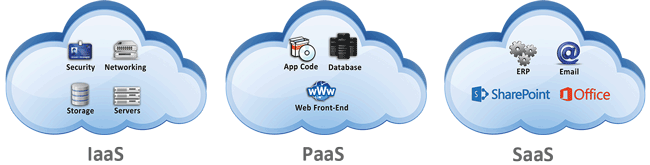
\includegraphics[width=8cm]{./service.png}
 \caption{Cloud Computing - Servcice Models \label{fig:Cloud Computing - Servcice Models} }
\end{figure}

\end{frame}

\begin{frame}{Cloud Computing - Deployment Model }

We can deploy the cloud in various ways.

\begin{itemize}
\item Public Cloud
\item Private Cloud
\item Hybrid cloud
\end{itemize}

\begin{figure}[H]
 \centering
 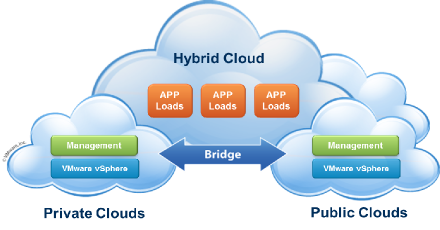
\includegraphics[width=5cm]{./model.png}
 \caption{Cloud Computing - Deployment Models \label{fig:model} }
\end{figure}
\end{frame}

\section{Private Clouds}
\begin{frame}{Private Clouds -- Introduction}

As per our concern we mainly focused about private clouds inorder to ensure Organizational data security \& High resource utilization

\hspace{4cm}\\

\textbf{``Private Cloud''} \\ 
\hspace{16mm} -- \textit{It is one of the cloud deployment model where the resources of small or medium organization are united and cattered to users of the that organization or outsourced through internet.} 

\end{frame}

\begin{frame}{Private Clouds -- Open Soruce Tools}

We can construct private cloud using some open source tools like Openstack, Cloudstack, OpenNebula. \\

\hspace{4cm} 

We can use this private cloud to deploy various services like Departmental Websites, Notice Boards, Events portal, High Computational Virtual Machines for Virtual Labs, High Performance Computing, Big data analytics.
\begin{figure}[H]
 \centering
 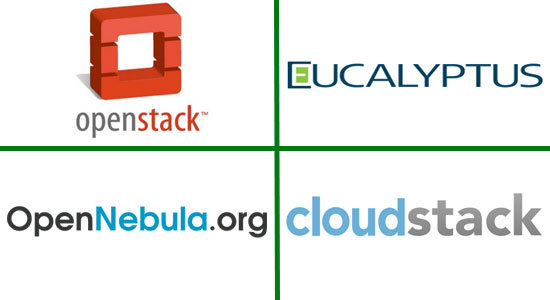
\includegraphics[width=5cm]{./cloud.jpg}
 \caption{Private Cloud - Open source tools \label{fig:cloud} }
\end{figure}

\end{frame}

\section{Questions?}
\begin{frame}{Questions?}
\centering
Questions ?
\end{frame}


\begin{frame}{One word to say ..}
Thank you
\end{frame}

\end{document}